\section{Mengen}
\begin{definition}[Menge]
Eine \emph{Menge} ist eine Zusammenfassung von unterscheidbaren Objekten. Diese Objekte heißen \emph{Element} der Menge.
\end{definition}

Eine Menge bezeichnet man mit einem lateinischen Buchstaben ($A$, $B$, $C$, \dots) und ein Element mit einem lateinischen Kleinbuchstaben ($a$, $b$, $c$, \dots).

Sei $M$ eine Menge und $x$ ein Objekt. Wenn $x$ ein Element von $M$ ist, schreibt man $x \in M$. Wenn $x$ kein Element von $M$ ist, schreibt man $x \notin M$. Es muss eindeutig feststellbar sein, ob $x$ Element $M$ ist oder nicht.

Es gibt verschiedene Möglichkeiten eine Menge zu definieren:
\begin{enumerate}
\item Durch Aufzählung
	\begin{align*}
	A &\ceq \gk{\tx{blau}, \tx{gelb}, \tx{rot}}\\
	B &\ceq \gk{\tx{Regensburg}, \tx{München}, \tx{Hamburg}, \tx{Berlin}}
	\end{align*}
\item Durch Beschreibung
	\begin{align*}
	C &\ceq \gk{x \vert x \tx{ ist durch $2$ teilbar}}\\
	D &\ceq \gk{x \vert x \tx{ ist eine deutsche Stadt}}\\
	E &\ceq \gk{x \vert x < 5}
	\end{align*}
\end{enumerate}
\begin{note}
Es sind nicht immer beide Varianten der Definition einer Menge möglich \ac{bzw.} sinnvoll.
\end{note}

\begin{note}
\enq{\ceq} bedeutet, dass die linke Seite durch die rechte Seite definiert wird.
\end{note}

\begin{example}[Bekannte Mengen]
\begin{align*}
\N &= \gk{x \vert x \tx{ ist eine natürliche Zahl}} = \gk{1, 2, 3, 4, \dots}\\
\N_0 &= \gk{0, 1, 2, 3, 4, \dots}\\
\Z &= \gk{x \vert x \tx{ ist eine ganze Zahl}} = \gk{\dots, -3, -2, -1, 0, 1, 2, 3, \dots} = \gk{0, \pm 1, \pm 2, \pm 3, \dots}\\
\Q &= \gk{x \vert x \tx{ ist eine rationale Zahl}} = \gk{\left.\frac{p}{q} \right| p \in \Z \tx{ und } q \in \N}\\
\R &= \gk{x \vert x \tx{ ist eine reelle Zahl}}
\end{align*}
\end{example}

\begin{definition}[Leere Menge]
Nach der Definition für Menge gibt es genau eine Menge, die \emph{keine Elemente} enthält. Diese Menge nennt man \emph{leere Menge} und schreibt $\emptyset$ oder $\gk{}$.
\end{definition}

\begin{definition}[(Echte) Teilmenge, (Echte) Obermenge]
Eine Menge $B$ heißt \emph{Teilmenge} von $A \rk{B \subseteq A}$, falls alle Elemente $x$ von $B$ auch Elemente von $A$ sind. $B$ heißt \emph{echte Teilmenge} von $A$, falls $B$ Teilmenge von $A$ und mindestens ein Element $y$ von $A$ existiert, das nicht in $B$ ist. Manschreibt dann $B \subset A$.\\
Wenn $B$ eine echte Teilmenge von $A$ ist, dann ist $A$ eine \emph{(echte) Obermenge} von $B$, geschrieben $A \supseteq B$ \ac{bzw.} $A \supset B$.
\end{definition}

\begin{example}
$\emptyset \subset \N \subset \N_0 \subset \Z \subset \Q \subset \R$
\end{example}

\begin{definition}[Mengenoperationen]
Seien $A$ und $B$ beliebige Mengen und $M$ eine Menge mit $A \subseteq M$ und $B \subseteq M$.
\begin{enumerate}
\item Der (Durch-)\emph{Schnitt} von $A$ und $B$ (siehe Abbildung~\vref{fig:Beispiel_fuer_Schnitt_zweier_Mengen}) wird definiert durch:
	\[A \cap B \ceq \gk{x \vert x \in A \tx{ und } x \in B}\]
	\begin{figure}[htb]
	\centering
	\input{pictures/2009.10.06-IMG1.tex}
	\caption{Beispiel für einen Schnitt zweier Mengen}
	\label{fig:Beispiel_fuer_Schnitt_zweier_Mengen}
	\end{figure}

\item Die \emph{Vereinigung} von $A$ und $B$ (siehe Abbildung~\vref{fig:Beispiel_fuer_Vereinigung_zweier_Mengen}) wird definiert durch:
	\[A \cup B \ceq \gk{x \vert x \in A \tx{ oder } x \in B}\]
	\begin{figure}[htb]
	\centering
	\input{pictures/2009.10.06-IMG2.tex}
	\caption{Beispiel für eine Vereinigung zweier Mengen}
	\label{fig:Beispiel_fuer_Vereinigung_zweier_Mengen}
	\end{figure}

\item Die \emph{Differenz} von $A$ und $B$ (siehe Abbildung~\vref{fig:Beispiel_fuer_Differenz_zweier_Mengen}) wird definiert durch:
	\[A \backslash B \ceq \gk{x \vert x \in A \tx{ und } x \notin B}\]
	\begin{figure}[htb]
	\centering
	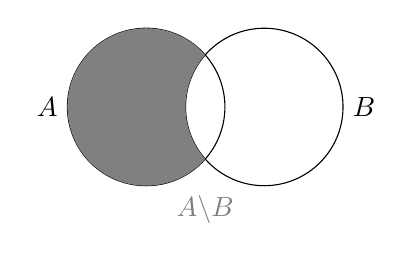
\begin{tikzpicture}
\def\firstcircle{(0,0) circle (1)}
\def\secondcircle{(1.5,0) circle (1)}

\draw \firstcircle;
\draw \secondcircle;

\node at (-1,0) [left] {$A$};
\node at (2.5,0) [right] {$B$};

\begin{scope}[even odd rule]% first circle without the second
\clip \secondcircle (-1,1) rectangle (2.5,-1);
\fill[gray] \firstcircle;
\end{scope}

\node[color=gray] at (0.75,-1) [below] {$A \backslash B$};
\end{tikzpicture}

	\caption{Beispiel für die Differenz zweier Mengen}
	\label{fig:Beispiel_fuer_Differenz_zweier_Mengen}
	\end{figure}

\item Die \emph{symmetrische Differenz} von $A$ und $B$ (siehe Abbildung~\vref{fig:Beispiel_fuer_symmetrische_Differenz_zweier_Mengen}) wird definiert durch:
	\[A \triangle B \ceq \rk{A \backslash B} \cup \rk{B \backslash A} = \rk{A \cup B} \backslash \rk{A \cap B}\]
	\begin{figure}[htb]
	\centering
	\input{pictures/2009.10.06-IMG4.tex}
	\caption{Beispiel für die symmetrische Differenz zweier Mengen}
	\label{fig:Beispiel_fuer_symmetrische_Differenz_zweier_Mengen}
	\end{figure}

\item Das \emph{Komplement} von $A$ bezüglich $M$ (siehe Abbildung~\vref{fig:Beispiel_fuer_Komplement_zweier_Mengen}) wird definiert durch:
	\[\bar{A} \tx{ oder } A^{\mathcal{C}} \ceq \gk{x \in M \vert x \notin A} = \gk{x \vert x \in M \tx{ und } x \notin A} = M \backslash A\]
	\begin{figure}[htb]
	\centering
	\input{pictures/2009.10.06-IMG5.tex}
	\caption{Beispiel für das Komplement zweier Mengen}
	\label{fig:Beispiel_fuer_Komplement_zweier_Mengen}
	\end{figure}

\item Die \emph{Produktmenge}, auch kathetisches Produkt genannt, der Mengen $A$ und $B$ (siehe Abbildung~\vref{fig:Beispiel_fuer_Produktmenge}) wird definiert durch:
	\[A \times B \ceq \gk{\rk{a, b} \vert a \in A \tx{ und } b \in B}\]
	\begin{figure}[htb]
	\centering
	\begin{tabular}{ccccccc}
&&& \large{$B = $} &&\\
&& $b_1$ & $b_2$ & \dots & $b_n$\\
&$a_1$& \textcolor{gray}{$\rk{a_1, b_1}$} & \textcolor{gray}{$\rk{a_1, b_2}$} & \textcolor{gray}{\dots} & \textcolor{gray}{$\rk{a_1, b_n}$}\\
\large{$A =$} &$a_2$   & \textcolor{gray}{$\rk{a_2, b_1}$} & \textcolor{gray}{$\rk{a_2, b_2}$} & \textcolor{gray}{\dots} & \textcolor{gray}{$\rk{a_2, b_n}$} & \textcolor{gray}{\large{$= A \times B$}}\\
&\vdots & \textcolor{gray}{\vdots}& \textcolor{gray}{\vdots}& \textcolor{gray}{\vdots}& \textcolor{gray}{\vdots}\\
&$a_n$& \textcolor{gray}{$\rk{a_n, b_1}$} & \textcolor{gray}{$\rk{a_n, b_2}$} & \textcolor{gray}{\dots} & \textcolor{gray}{$\rk{a_n, b_n}$}
\end{tabular}

	\caption{Beispiel für die Produktmenge}
	\label{fig:Beispiel_fuer_Produktmenge}
	\end{figure}
	\begin{example}
	$A = \gk{0, 1, 2}, B = \gk{1, 2}$
	\[A \times B = \gk{\rk{0,1}, \rk{0,2}, \rk{1,1}, \rk{1,2}, \rk{2,1}, \rk{2,2}}\]
	Graphische Darstellung siehe Abbildung~\vref{fig:Beispiel_fuer_Produktmenge_2}.
	\begin{figure}[htb]
	\centering
	\begin{tikzpicture}
\draw (0,0) node[left] {$1$} -- (4,0);
\draw (0,2) node[left] {$2$} -- (4,2);
\draw (0,0) node[below] {$0$} -- (0,2);
\draw (2,0) node[below] {$1$} -- (2,2);
\draw (4,0) node[below] {$2$} -- (4,2);
\end{tikzpicture}

	\caption{Graphische Darstellung einer Produktmenge}
	\label{fig:Beispiel_fuer_Produktmenge_2}
	\end{figure}
	\end{example}
\end{enumerate}

\label{def:1.4}
\end{definition}

\begin{note}
Die Bildchen in Definition~\vref{def:1.4} nennt man Venn-Diagramme.
\end{note}

\begin{theorem}[Rechenregeln für $\cap$, $\cup$, $\bar{M}$]
Seien $A$, $B$, $C$ beliebige Mengen und $M$ eine Menge mit $A, B, C \subseteq M$. Für die verschiedenen Gesetze siehe Tabelle~\vref{tab:Rechenregeln_fuer_Operationen_cap-cup-bar}.
\begin{table}[htb]
\centering
\begin{tabular}{cc}
\toprule
\multicolumn{2}{c}{\emph{Assoziativgesetze}}\\
$\rk{A \cap B} \cap C = A \cap \rk{B \cap C}$ & $\rk{A \cup B} \cup C = A \cup \rk{B \cup C}$\\
\midrule

\multicolumn{2}{c}{\emph{Kommutativgesetze}}\\
$A \cap B = B \cap A$ & $A \cup B = B \cup A$\\
\midrule

\multicolumn{2}{c}{\emph{Distributivgesetze}}\\
$A \cap \rk{B \cup C} = \rk{A \cap B} \cup \rk{A \cap C}$ & $A \cup \rk{B \cap C} = \rk{A \cup B} \cap \rk{A \cup C}$\\
\midrule

\multicolumn{2}{c}{\emph{Idempotenzgesetze}}\\
$A \cap A = A$ & $A \cup A = A$\\
\midrule

\multicolumn{2}{c}{\emph{Absorptionsgesetze}}\\
$A \cap \rk{B \cup A} = A$ & $A \cup \rk{B \cap A} = A$\\
\midrule

\multicolumn{2}{c}{\emph{Null und Eins}}\\
$A \cap \emptyset = \emptyset$ & $A \cup \emptyset = A$\\
$A \cap M = A$ & $A \cup M = M$\\
\midrule

\multicolumn{2}{c}{\emph{Komplementgesetze}}\\
$A \cap \bar{A} = \emptyset$ & $A \cup \bar{A} = M$\\
\midrule

\multicolumn{2}{c}{\emph{Gesetze von de Morgan}}\\
$\overline{A \cap B} = \bar{A} \cup \bar{B}$ & $\overline{A \cup B} = \bar{A} \cap \bar{B}$\\
\bottomrule
\end{tabular}
\label{tab:Rechenregeln_fuer_Operationen_cap-cup-bar}
\caption{Rechenregeln für Operationen $\cap$, $\cup$ und $\bar{M}$}
\end{table}
\end{theorem}

\begin{proof}[Exemplarisch zum Distributivgesetz]
\ac{z.z.}
\[A \cap \rk{B \cup C} = A \cap B \cup A \cap C\]
Für die Zugehörigen Venn-Diagramme siehe Abbildungen~\vref{fig:2009.10.07-IMG3} und \vref{fig:2009.10.07-IMG4}.
\begin{figure}[htb]
\centering
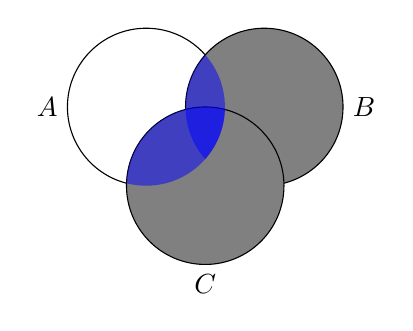
\begin{tikzpicture}
\def\firstcircle{(0,0) circle (1)}
\def\secondcircle{(1.5,0) circle (1)}
\def\thirdcircle{(0.75,-1) circle (1)}

\node at (-1,0) [left] {$A$};
\node at (2.5,0) [right] {$B$};
\node at (0.75,-2) [below] {$C$};

\draw \firstcircle;
\draw[fill=gray] \secondcircle;
\draw[fill=gray] \thirdcircle;

\begin{scope}
\clip \firstcircle;
\clip \secondcircle;
\fill[semitransparent,blue] \secondcircle;
\end{scope}
\begin{scope}
\clip \firstcircle;
\clip \thirdcircle;
\fill[semitransparent,blue] \thirdcircle;
\end{scope}
\end{tikzpicture}

\caption{$A \cap \rk{B \cup C}$}
\label{fig:2009.10.07-IMG3}
\end{figure}

\begin{figure}[htb]
\centering
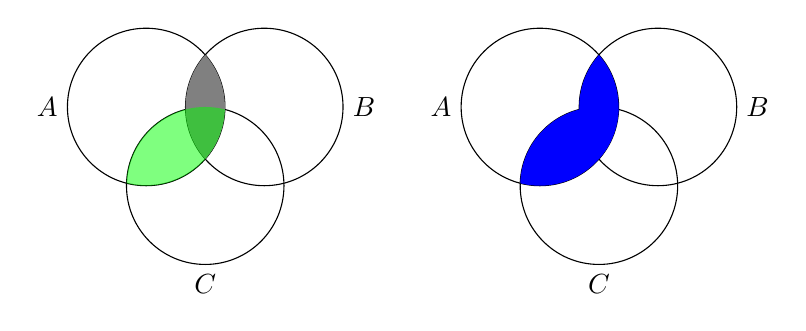
\begin{tikzpicture}
\begin{scope}
\def\firstcircle{(0,0) circle (1)}
\def\secondcircle{(1.5,0) circle (1)}
\def\thirdcircle{(0.75,-1) circle (1)}

\node at (-1,0) [left] {$A$};
\node at (2.5,0) [right] {$B$};
\node at (0.75,-2) [below] {$C$};

\draw \firstcircle;
\draw \secondcircle;
\draw \thirdcircle;

\begin{scope}
\clip \firstcircle;
\clip \secondcircle;
\fill[gray] \secondcircle;
\end{scope}
\begin{scope}
\clip \firstcircle;
\clip \thirdcircle;
\fill[semitransparent,green] \thirdcircle;
\end{scope}
\end{scope}

\node at (3.25,-0.75) {\Large \Ra};

\begin{scope}
\def\firstcircle{(5,0) circle (1)}
\def\secondcircle{(6.5,0) circle (1)}
\def\thirdcircle{(5.75,-1) circle (1)}

\node at (4,0) [left] {$A$};
\node at (7.5,0) [right] {$B$};
\node at (5.75,-2) [below] {$C$};

\draw \firstcircle;
\draw \secondcircle;
\draw \thirdcircle;

\begin{scope}
\clip \firstcircle;
\clip \secondcircle;
\fill[blue] \secondcircle;
\end{scope}
\begin{scope}
\clip \firstcircle;
\clip \thirdcircle;
\fill[blue] \thirdcircle;
\end{scope}
\end{scope}
\end{tikzpicture}

\caption{\textcolor{blue}{$\rk{\textcolor{gray}{A \cap B}} \cup \rk{\textcolor{green}{A \cap C}}$}}
\label{fig:2009.10.07-IMG4}
\end{figure}
\end{proof}

\begin{definition}~
\begin{enumerate}
\item Die Mengen $A$ und $B$ heißen \emph{disjunkt} falls $A \cap B = \emptyset$.
\item Für den Schnitt der Mengen $A_1$, $A_2$, \dots, $A_n$ schreibt man \[A_1 \cap A_2 \cap \dots \cap A_n \eqc \bigcap_{j = 1}^{n} A_j\]
\item Für die Vereinigung der Mengen $A_1$, $A_2$, \dots, $A_n$ schreibt man \[A_1 \cup A_2 \cup \dots \cup A_n \eqc \bigcup_{j = 1}^{n} A_j\]
\item Ist $M$ eine endliche Menge oder eine abzählbare Menge (\ac{z.B.} \N, \Z, \Q aber nicht \R) dann nennt man die Menge aller Teilmengen von $M$ die Potenzmenge $\pmeng{M}$.
\end{enumerate}
\end{definition}

\begin{note}
Hat die Menge $M$ genau $n$ Element, dann hat die Potzenzmenge $\pmeng{M}$ genau $2^n$ Elemente.
\end{note}
